\section{Background}\label{sec:background}

This case study is performed at 30MHz, specifically within the context of their software platform. This section describes the company (30MHz), their software platform (the dashboard) and the problem that is solved by the case study.

\subsection{The Company}\label{sec:bg-thecompany}
30MHz is a technology company in the agriculture industry. They offer sensors that collect various types of data, all within the context of agriculture. For example temperature, humidity, air pressure etc. They also provide their customers with a dashboard that allows them to view the collected data. 30MHz has a number of so-called partners. These partners are consultancies in the field of agriculture (among others). They supply 30MHz with additional customers by suggesting their clients to become customers of 30MHz as well.

30MHz supplies their customers with the so-called dashboard. An example of which can be seen in Figure~\ref{fig:bg-dashboard}. It is the central location where any customer can view their data. This dashboard is a web app that, as of this case study, is using Angular 10. Data is fetched from a backend and the various types of data are displayed in different ways using so-called widgets. An example of a widget is a chart that displays the value of the data over time.

\begin{figure}[h]
	\caption{Widgets on the 30MHz dashboard}
	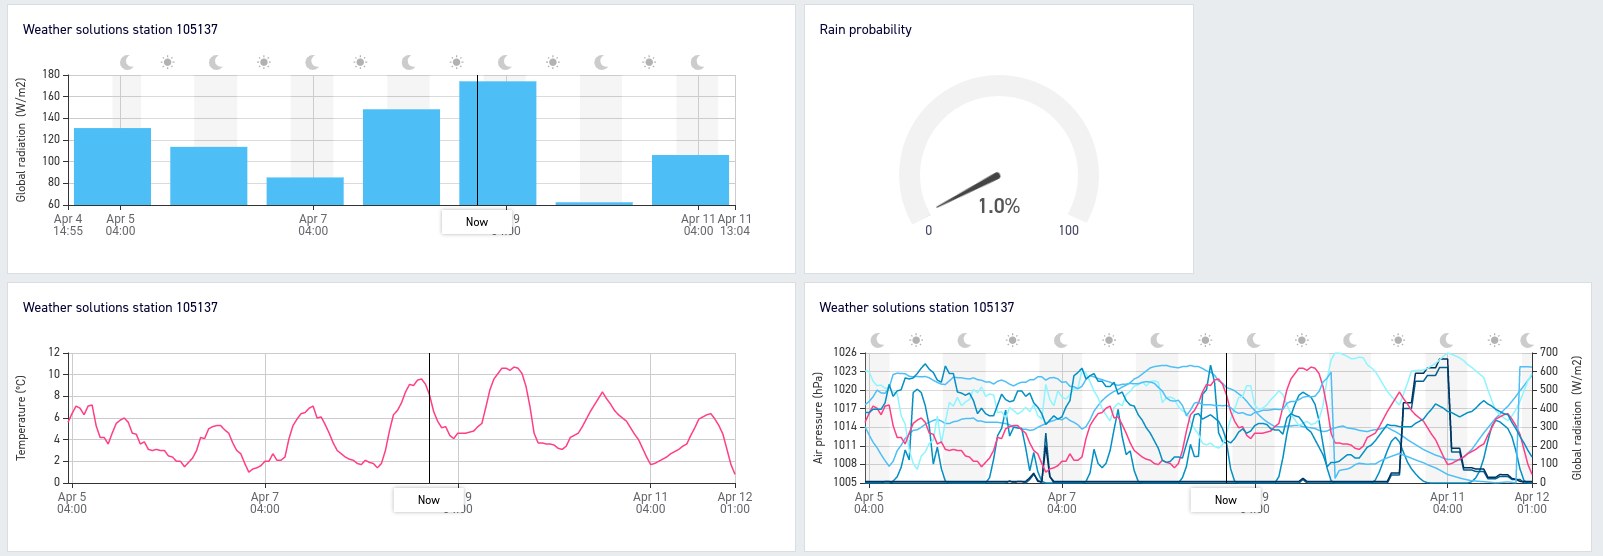
\includegraphics[width=\columnwidth]{figures/background/dashboard.png}
	\label{fig:bg-dashboard}
	\centering
\end{figure}

\subsubsection{Apps}\label{sec:bg-apps}
The large amounts of data collected by 30MHz can be utilized in many ways. Companies with domain knowledge and expertise in certain areas (such as the partners) can use it to provide customers with new insights and information that simple graphs can not. Because 30MHz itself does not have this domain knowledge and does not have the resources to create every single possible implementation of this knowledge (in the form of a widget or page in the dashboard), they decided to allow 3rd party developers to develop them instead. In practice, these will be built by the partners, and will be provided to customers of 30MHz for a fee through a marketplace. There are currently two implementations:

\begin{itemize}
	\item \emph{Widgets:} Widgets in the dashboard that take data from one or more sensors and display it. These are made to provide information at a quick glance and are fairly small, as can be seen in Figure~\ref{fig:bg-dashboard}. An example would be a new way to display sun data by showing a sun if the plants are able to grow (it's daytime) and a moon if they're not (it's nighttime).
	\item \emph{Apps:} Full pages in the dashboard web app. These fill the entire screen (bar some 30MHz branding) and can provide more rich and interactive experiences. An example would be a page where clients of a partner can tune some parameters (such as number of crops, amount of watering) and see a prediction of their revenue. This prediction can be based (in part) on sensor data.
\end{itemize}

Since these apps will essentially be pages in the 30MHz dashboard, and will feel like part of the platform, it is important that they follow the same design style and principles as the rest of the dashboard. This ensures that users are familiar with the apps and that visual consistency across the platform is not broken. This concept has been applied many times. For example on Google's Android through Material Design~\footnote{\url{https://material.io/}}, Apple's design on iOS~\footnote{\url{https://developer.apple.com/design/}}, Zendesk Garden~\footnote{\url{https://garden.zendesk.com/}} and many more. Importantly, these companies all provide their app developers with a set of components in order to help them maintain their design language. Such a set of components is generally referred to as a UI library. Similarly, 30MHz wants to provide their 3rd party app developers with a UI library as well. There already is an internal set of components that cover the basic set of UI components (buttons, an input, a date picker etc), but since these are largely interwoven with other internal code, their source code can not just be provided to 3rd party developers. They have also been written in Angular~\footnote{\url{https://angular.io/}}, meaning that any developers who wish to develop their app in a different JavaScript (JS) framework are unable to do so. Looking at the most popular web frameworks in the latest Stack Overflow Developer Survey~\cite{stack-overflow-dev-survey} (2020 as of the writing of this paper), we can conclude that the chance that a developer wishes to use a different JS framework is quite large. In order to still provide developers with a UI library, there are two options.

\begin{itemize}
	\item Write components from scratch in a framework-agnostic format and provide them to developers. Then keep them up to date with the internal set of components by changing one as the other changes.
	\item Set up automatic conversion from the set of internal components to a framework-agnostic format.
\end{itemize}

The obvious problem with the first option is that you're basically maintaining two separate copies of very similar code. This causes a number of issues. Firstly the time spent maintaining a component is doubled. Additionally, feature differences between the Angular framework and the framework-agnostic format we choose are going to lead to problems. Some things that work in Angular might need workarounds in the other format and the other way around. Another issue with this option is that the components have to be written entirely from scratch. While this would be manageable for simple components such as buttons, this is unfeasible for more complex components. One of which is the chart component. This component is important to have in the 30MHz design library, seeing as it is able to display the sensor data. However, the source code for the chart alone is already 500 lines long, most of which are tightly integrated with the rest of the platform. Through all of its references, the chart component references about half of the source files in the dashboard. Rewriting all of this in another framework is completely unfeasible and not worth the effort, leading us to explore the second option.

While the second option is not an easy one and it will likely be a very complex process to set up, it is one that will scale a lot better. Once it is set up, any new components will be automatically converted and any changes will be propagated automatically. In the long run, this should save a lot of time. This is the option 30MHz eventually decided on. However, a framework-agnostic format needs to be chosen to facilitate this process.

\subsection{Web Components}\label{sec:bg-webcomponents}
When it comes to choosing a framework-agnostic format for a UI library, there are very few options. Looking at the literature, we find Quid, a DSL for generating components in various frameworks~\cite{molina2019quid}. It currently supports Web Components~\footnote{\url{https://developer.mozilla.org/en-US/docs/Web/Web_Components}}, Stencil~\footnote{\url{https://stenciljs.com/}}, Angular and Polymer~\footnote{\url{https://www.polymer-project.org/}}. While this is fairly impressive, the authors do mention it should only be used for rapid prototyping. Since it only supports a fairly small set of supported frameworks and it has the problem of requiring a DSL which the Angular code would have to be converted to, this is not a great fit for us.

This brings us to the other option, namely Web Components. Web Components (also known as Custom Elements) are a technology proposed in 2013~\cite{customelements-initial} and implemented in major browsers in 2018~\cite{webcomponents-support}. It allows for the creation of custom HTML elements using JavaScript. These elements can then be used like regular HTML elements. Since every JS framework has support for native HTML elements and almost every framework has full support for Web Components~\cite{custom-elements-everyhwere}, we can cover most JS frameworks by using Web Components as our target format.

\subsection{Angular Elements}\label{sec:bg-angularelements}
To perform the conversion of Angular components to Web Components, we will be using Angular Elements~\footnote{\url{https://angular.io/guide/elements}}. Angular Elements is a JS package published by the developers of Angular that allows the conversion of Angular components to Web Components. Angular apps are normally mounted to the DOM by the user through a call to the \(bootstrapModule\) function. After this call, the bootstrap component is mounted to the DOM, after which child components are rendered within its root recursively. Angular Elements works slightly different. Components registered as Web Components through Angular Elements are instead rendered whenever an HTML element with the registered tag is added to the DOM\@. When this happens, a new root is created in place of this new HTML element. Instead of there being a single root in which everything is rendered (as is the case in a normal Angular app), components are all rendered in their own local root. We will be using Angular Elements for the conversion to Web Components in this case study.

\begin{figure}[h]
	\caption{An example of a component that provides type hints}
	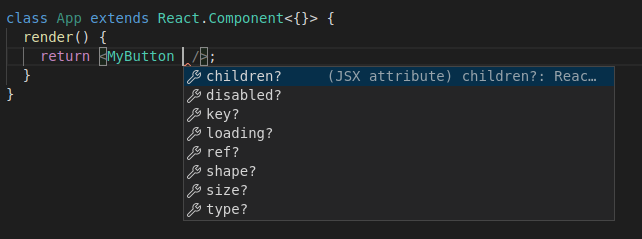
\includegraphics[width=\columnwidth]{figures/background/hinting.png}
	\label{fig:bg-hinting}
	\centering
\end{figure}

\begin{figure}[h]
	\caption{An example of a component without type hints}
	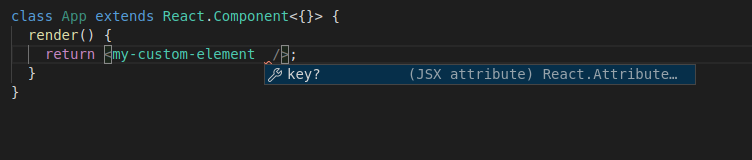
\includegraphics[width=\columnwidth]{figures/background/no-hinting.png}
	\label{fig:bg-no-hinting}
	\centering
\end{figure}

\subsection{Javascript frameworks}\label{sec:bg-jsframeworks}
While converting components to Web Components makes them usable in most JS frameworks, they do not provide a perfect experience. The first problem is them not being perfectly usable in every JS framework. As of the writing of this paper, there are still some issues preventing them from working completely in React JS~\footnote{\url{https://reactjs.org/}}. The second problem is that they are not native to JS frameworks, and as such do not integrate very well with the tooling provided by the framework. An example of type hinting provided by the framework and editor can be seen in Figure~\ref{fig:bg-hinting}. Compared to Figure~\ref{fig:bg-no-hinting}, which shows a component with no type hinting, Figure~\ref{fig:bg-hinting} provides the developer with much more information and shows them what options are available to them. Instead of having to search the web for the available properties, they are provided by the element's source code and displayed by the framework tooling and editor. In order to provide developers with proper tooling and type hinting for components, we will provide what we'll call a wrapper for each framework that either provides this tooling or does not support Web Components fully. This wrapper is written in the language the framework which it is targeting provides, and as such allows the framework to infer information from its source code. Under the hood this wrapper still makes use of the Web Components to render the components in the UI library, but this wrapper serves as glue code between the framework and the Web Components. By combining the two steps of converting the original Angular components to Web Components, and the Web Components to wrappers for frameworks, we are able to provide developers with an experience that is native to their framework, regardless of the fact that the original source code was written in Angular.